\begin{problem}{자벌레 세기}{standard input}{standard output}{2 seconds}{1024 megabytes}

$N$개의 정점으로 구성된 트리가 있습니다. 트리는 간선에 방향이 없는 연결된 그래프로, 각 정점에서 다른 정점으로 가는 최단 경로가 유일합니다.

어떤 $6$개의 \textbf{서로 다른} 정점 $(u,v,w,x,y,z)$가 다음 조건을 모두 만족할 경우 그러한 $6$개의 정점으로 구성된 그래프를 \textbf{자벌레}라고 합니다.

\begin{itemize}
\item $u$와 $v$가 간선으로 직접 연결되어 있습니다.
\item $w,x,y,z$ 중 $2$개는 $u$와, 나머지 $2$개는 $v$와 간선으로 직접 연결되어 있습니다.
\end{itemize}

이때, 두 자벌레 $A$와 $B$에 대해, $A$에 포함되어 있으면서 $B$에 포함되지 않은 정점이 존재한다면 $A$와 $B$는 \textbf{서로 다른} 자벌레로 취급합니다.

예를 들어, 다음 그림에 주어진 트리에 대해, 빨간색으로 색칠된 간선으로 연결된 $6$개의 정점이 자벌레의 예시입니다.

\begin{center}
  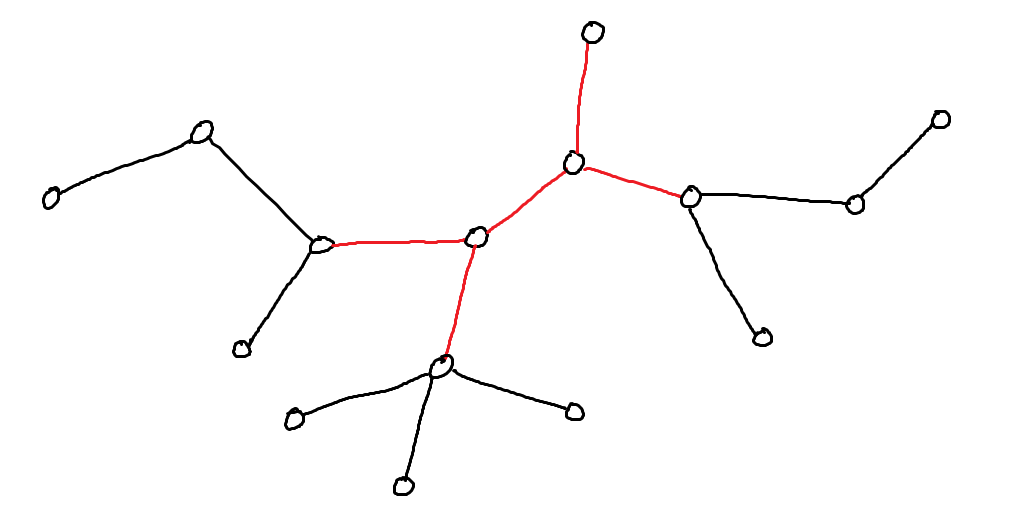
\includegraphics[scale=0.5]{stickbug.png}
\end{center}

위의 트리에는 서로 다른 자벌레가 총 $6$개 존재합니다.

입력으로 주어진 트리에 대해서, 트리에 존재하는 서로 다른 자벌레의 수를 구하는 프로그램을 작성해 주세요.

\InputFile
첫 번째 줄에 트리를 구성하는 정점의 개수 $N$이 주어집니다.

두 번째 줄부터 $N-1$개의 줄에 걸쳐 각각의 간선이 연결하는 두 정점의 번호 $u_i$, $v_i$가 공백으로 구분되어 주어집니다.



\OutputFile
입력으로 주어진 트리에 존재하는 서로 다른 자벌레의 수를 한 줄에 출력합니다.

\Scoring
제한:

\begin{itemize}
\item $2 \le N \le 300\,000$
\item $1 \le u_i,v_i \le N$
\item $u_i \neq v_i$
\item 주어진 그래프는 올바른 트리임이 보장됩니다.
\item \textbf{주어진 트리에 존재하는 서로 다른 자벌레의 수는 $10^{18}$을 초과하지 않음이 보장됩니다.}
\end{itemize}

서브태스크:

\begin{tabular}{|l|l|l|} \hline
  \textbf{번호} & \textbf{배점} & \textbf{제한} \\ \hline
  1 & 13 & $N \le 300$ \\ \hline
  2 & 37 & $N \le 3000$ \\ \hline
  3 & 7 & 각 $1 \le i \le N-1$에 대해 $u_i=1$ 또는 $u_i=i$이며 $v_i=i+1$ \\ \hline
  4 & 43 & 추가 제한 없음 \\ \hline
\end{tabular}

\Example

\begin{example}
\exmpfile{example.01}{example.01.a}%
\end{example}

\end{problem}

